\section{Entity Relationship Diagram}
\subsection{Entities}
We will have six entities: user, post, question, answer, comment, and topic.

A user is an individual writing a post on Ask Us. The user entity will have five attributes: ID, name, email, password, and points. A user's points are the sum of all the points of all their posts. ID will be the primary key.

A post is anything a user writes. This can either be a question, answer, or comment. The post entity will only have an ID, which is the primary key.

Questions, answers, and comments will all have the following attributes, aside from the ones we will specify below. They will have a body, which is the main text that makes up that post. They will also have a count of the points that they have been awarded by users.

A question is what a user would post if he wanted to receive a solution to his inquiry. The question entity has other attribute called title, apart from the attributes listed above. Since it is a weak entity, its primary key is the post's ID.

An answer is what a user would post if he wanted to give a solution to a question. The answer entity has a boolean attribute called accepted, apart from the attributes listed above. Since it is a weak entity, its primary key is the post's ID.

A comment is a type of post, and is typically a short piece of text that a user writes beneath any other post. A comment itself has no other attributes, other than the ones above. Since it is a weak entity, its primary key is the post's ID.

A topic is a way for users to categorize their questions, thus getting better targeted responses. A user can also follow a topic of interest. The topic entity will have three attributes: ID, name, and description. ID will once again be the primary key.

\subsection{Relations}
A user can `follow' a topic. In this relation, there can be many topics a user can follow, but it is not mandatory for a user to follow any topic. In the same light, there can be topics followed by any number of users.

A user is related to the posts that they write, by writing either a question, an answer or a comment. In this relation, the user can write anywhere from many to no posts. However, a post must be written by exactly one user.

A user is also related to a post by voting on it. The vote relation is a many to many relation, in that a user can vote on many to no posts and a post can be voted on by many to no users.

The comment entity has two relations with the post entity. One relation is called belongs to. This relation represents the fact that a specific comment has a parent post (which may also be a comment). A post can optionally have many comments, but a comment must be a child of exactly one post.

The other relation is an inheritance relation. It is an identifying relation, and is labelled `is a' in figure \ref{erd}. In this relation, a particular comment is related to exactly one post, meaning that this comment entity `extends' that post, because they are in fact the same post. In this relation, a post does not necessarily have to be related to a comment, since not all posts are comments, but if it is, it must be related to exactly one comment.

Since a questions and answers are also types of post, they also have an inheritance relation between themselves and post. This relation is identical to the inheritance relation between comment and post.

Answers must also be related to the questions which they answer. A question can have zero to infinitely many answers, yet an answer must be related to exactly one question.

Lastly, questions are related to topics. A question must have at least one topic, and a topic can have zero or more questions related to it.

\subsection{Diagram}

Figure \ref{erd} shows the entity relationship diagram for the database we are to make for Ask Us.

\begin{figure}[p]
	\centering
	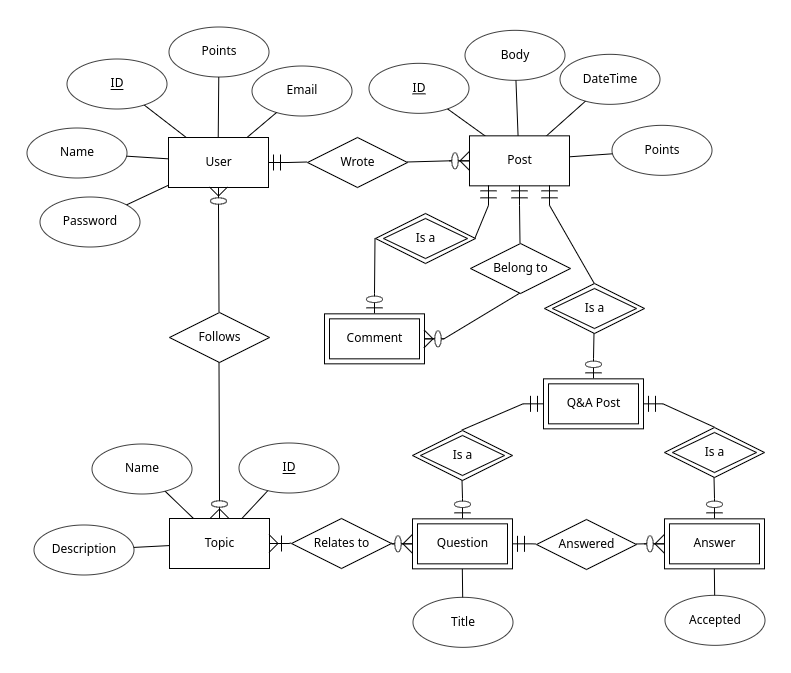
\includegraphics[width=\linewidth]{../../ERD/erd.png}
	\caption{An ERD for the database for Ask Us}
	\label{erd}
\end{figure}